\documentclass{article}
\usepackage{tikz}

\begin{document}

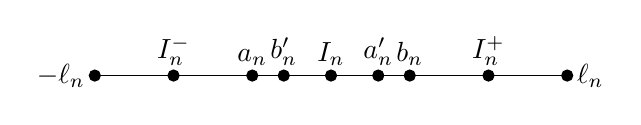
\begin{tikzpicture}[scale=2]
    % Draw the horizontal line
    \draw (-1.5,0) -- (1.5,0);
    
    % Mark the endpoints with labels
    \filldraw[black] (-1.5,0) circle (1pt) node[left] {$-\ell_n$};
    \filldraw[black] (1.5,0) circle (1pt) node[right] {$\ell_n$};
    
    % Mark the intervals and points
    \filldraw[black] (-1,0) circle (1pt) node[above] {$I_n^-$};
    \filldraw[black] (-0.5,0) circle (1pt) node[above] {$a_n$};
    \filldraw[black] (-0.3,0) circle (1pt) node[above] {$b'_n$};
    \filldraw[black] (0,0) circle (1pt) node[above] {$I_n$};
    \filldraw[black] (0.3,0) circle (1pt) node[above] {$a'_n$};
    \filldraw[black] (0.5,0) circle (1pt) node[above] {$b_n$};
    \filldraw[black] (1,0) circle (1pt) node[above] {$I_n^+$};
\end{tikzpicture}

\end{document}